\documentclass[]{article}
\usepackage{lmodern}
\usepackage{amssymb,amsmath}
\usepackage{ifxetex,ifluatex}
\usepackage{fixltx2e} % provides \textsubscript
\ifnum 0\ifxetex 1\fi\ifluatex 1\fi=0 % if pdftex
  \usepackage[T1]{fontenc}
  \usepackage[utf8]{inputenc}
\else % if luatex or xelatex
  \ifxetex
    \usepackage{mathspec}
  \else
    \usepackage{fontspec}
  \fi
  \defaultfontfeatures{Ligatures=TeX,Scale=MatchLowercase}
\fi
% use upquote if available, for straight quotes in verbatim environments
\IfFileExists{upquote.sty}{\usepackage{upquote}}{}
% use microtype if available
\IfFileExists{microtype.sty}{%
\usepackage{microtype}
\UseMicrotypeSet[protrusion]{basicmath} % disable protrusion for tt fonts
}{}
\usepackage[margin=1in]{geometry}
\usepackage{hyperref}
\hypersetup{unicode=true,
            pdftitle={HTML Dokumente Präsentationen und Dashboards},
            pdfauthor={Jan-Philipp Kolb},
            pdfborder={0 0 0},
            breaklinks=true}
\urlstyle{same}  % don't use monospace font for urls
\usepackage{color}
\usepackage{fancyvrb}
\newcommand{\VerbBar}{|}
\newcommand{\VERB}{\Verb[commandchars=\\\{\}]}
\DefineVerbatimEnvironment{Highlighting}{Verbatim}{commandchars=\\\{\}}
% Add ',fontsize=\small' for more characters per line
\usepackage{framed}
\definecolor{shadecolor}{RGB}{248,248,248}
\newenvironment{Shaded}{\begin{snugshade}}{\end{snugshade}}
\newcommand{\KeywordTok}[1]{\textcolor[rgb]{0.13,0.29,0.53}{\textbf{#1}}}
\newcommand{\DataTypeTok}[1]{\textcolor[rgb]{0.13,0.29,0.53}{#1}}
\newcommand{\DecValTok}[1]{\textcolor[rgb]{0.00,0.00,0.81}{#1}}
\newcommand{\BaseNTok}[1]{\textcolor[rgb]{0.00,0.00,0.81}{#1}}
\newcommand{\FloatTok}[1]{\textcolor[rgb]{0.00,0.00,0.81}{#1}}
\newcommand{\ConstantTok}[1]{\textcolor[rgb]{0.00,0.00,0.00}{#1}}
\newcommand{\CharTok}[1]{\textcolor[rgb]{0.31,0.60,0.02}{#1}}
\newcommand{\SpecialCharTok}[1]{\textcolor[rgb]{0.00,0.00,0.00}{#1}}
\newcommand{\StringTok}[1]{\textcolor[rgb]{0.31,0.60,0.02}{#1}}
\newcommand{\VerbatimStringTok}[1]{\textcolor[rgb]{0.31,0.60,0.02}{#1}}
\newcommand{\SpecialStringTok}[1]{\textcolor[rgb]{0.31,0.60,0.02}{#1}}
\newcommand{\ImportTok}[1]{#1}
\newcommand{\CommentTok}[1]{\textcolor[rgb]{0.56,0.35,0.01}{\textit{#1}}}
\newcommand{\DocumentationTok}[1]{\textcolor[rgb]{0.56,0.35,0.01}{\textbf{\textit{#1}}}}
\newcommand{\AnnotationTok}[1]{\textcolor[rgb]{0.56,0.35,0.01}{\textbf{\textit{#1}}}}
\newcommand{\CommentVarTok}[1]{\textcolor[rgb]{0.56,0.35,0.01}{\textbf{\textit{#1}}}}
\newcommand{\OtherTok}[1]{\textcolor[rgb]{0.56,0.35,0.01}{#1}}
\newcommand{\FunctionTok}[1]{\textcolor[rgb]{0.00,0.00,0.00}{#1}}
\newcommand{\VariableTok}[1]{\textcolor[rgb]{0.00,0.00,0.00}{#1}}
\newcommand{\ControlFlowTok}[1]{\textcolor[rgb]{0.13,0.29,0.53}{\textbf{#1}}}
\newcommand{\OperatorTok}[1]{\textcolor[rgb]{0.81,0.36,0.00}{\textbf{#1}}}
\newcommand{\BuiltInTok}[1]{#1}
\newcommand{\ExtensionTok}[1]{#1}
\newcommand{\PreprocessorTok}[1]{\textcolor[rgb]{0.56,0.35,0.01}{\textit{#1}}}
\newcommand{\AttributeTok}[1]{\textcolor[rgb]{0.77,0.63,0.00}{#1}}
\newcommand{\RegionMarkerTok}[1]{#1}
\newcommand{\InformationTok}[1]{\textcolor[rgb]{0.56,0.35,0.01}{\textbf{\textit{#1}}}}
\newcommand{\WarningTok}[1]{\textcolor[rgb]{0.56,0.35,0.01}{\textbf{\textit{#1}}}}
\newcommand{\AlertTok}[1]{\textcolor[rgb]{0.94,0.16,0.16}{#1}}
\newcommand{\ErrorTok}[1]{\textcolor[rgb]{0.64,0.00,0.00}{\textbf{#1}}}
\newcommand{\NormalTok}[1]{#1}
\usepackage{longtable,booktabs}
\usepackage{graphicx,grffile}
\makeatletter
\def\maxwidth{\ifdim\Gin@nat@width>\linewidth\linewidth\else\Gin@nat@width\fi}
\def\maxheight{\ifdim\Gin@nat@height>\textheight\textheight\else\Gin@nat@height\fi}
\makeatother
% Scale images if necessary, so that they will not overflow the page
% margins by default, and it is still possible to overwrite the defaults
% using explicit options in \includegraphics[width, height, ...]{}
\setkeys{Gin}{width=\maxwidth,height=\maxheight,keepaspectratio}
\IfFileExists{parskip.sty}{%
\usepackage{parskip}
}{% else
\setlength{\parindent}{0pt}
\setlength{\parskip}{6pt plus 2pt minus 1pt}
}
\setlength{\emergencystretch}{3em}  % prevent overfull lines
\providecommand{\tightlist}{%
  \setlength{\itemsep}{0pt}\setlength{\parskip}{0pt}}
\setcounter{secnumdepth}{0}
% Redefines (sub)paragraphs to behave more like sections
\ifx\paragraph\undefined\else
\let\oldparagraph\paragraph
\renewcommand{\paragraph}[1]{\oldparagraph{#1}\mbox{}}
\fi
\ifx\subparagraph\undefined\else
\let\oldsubparagraph\subparagraph
\renewcommand{\subparagraph}[1]{\oldsubparagraph{#1}\mbox{}}
\fi

%%% Use protect on footnotes to avoid problems with footnotes in titles
\let\rmarkdownfootnote\footnote%
\def\footnote{\protect\rmarkdownfootnote}

%%% Change title format to be more compact
\usepackage{titling}

% Create subtitle command for use in maketitle
\newcommand{\subtitle}[1]{
  \posttitle{
    \begin{center}\large#1\end{center}
    }
}

\setlength{\droptitle}{-2em}

  \title{HTML Dokumente Präsentationen und Dashboards}
    \pretitle{\vspace{\droptitle}\centering\huge}
  \posttitle{\par}
    \author{Jan-Philipp Kolb}
    \preauthor{\centering\large\emph}
  \postauthor{\par}
      \predate{\centering\large\emph}
  \postdate{\par}
    \date{8 Mai 2017}


\begin{document}
\maketitle

\subsection{\texorpdfstring{\href{https://rstudio-pubs-static.s3.amazonaws.com/27777_55697c3a476640caa0ad2099fe914ae5.html\#/}{\textbf{Präsentationen
- Rpres der einfachste
Weg}}}{Präsentationen - Rpres der einfachste Weg}}\label{prasentationen---rpres-der-einfachste-weg}

\begin{figure}
\centering

\includegraphics{figure/Rpresentations.PNG}
\caption{}
\end{figure}

\subsection{Eine erste Präsentation}\label{eine-erste-prasentation}

\begin{figure}
\centering
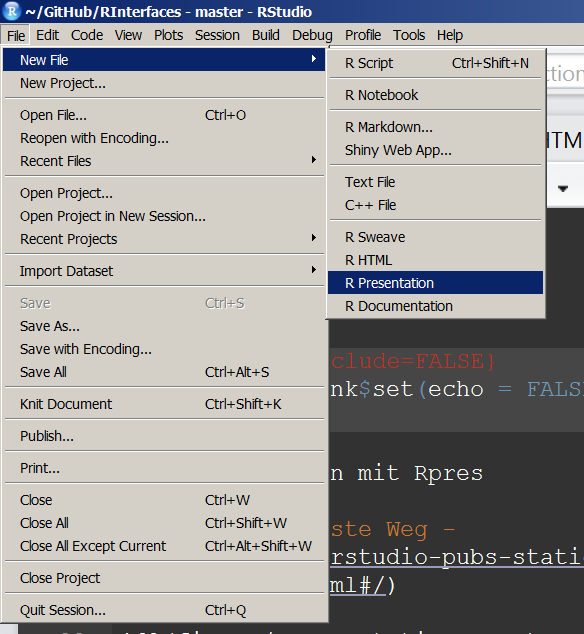
\includegraphics{figure/RpresStart.PNG}
\caption{}
\end{figure}

\subsection{Erste Daten eintragen}\label{erste-daten-eintragen}

\begin{itemize}
\tightlist
\item
  Für Vergessliche:
\end{itemize}

\begin{Shaded}
\begin{Highlighting}[]
\KeywordTok{date}\NormalTok{()}
\end{Highlighting}
\end{Shaded}

\begin{verbatim}
## [1] "Thu Oct 04 15:19:42 2018"
\end{verbatim}

\subsection{Eine Folie mit Formel}\label{eine-folie-mit-formel}

\begin{itemize}
\tightlist
\item
  Die Formel kann wie in LaTeX eingegeben werden
\end{itemize}

\begin{verbatim}
$$
\begin{equation}\label{eq2}
t_{i}=\sum\limits_{k=1}^{M_{i}}{y_{ik}}=M_{i}\bar{Y}_{i}. 
\end{equation}
$$
\end{verbatim}

\begin{figure}
\centering
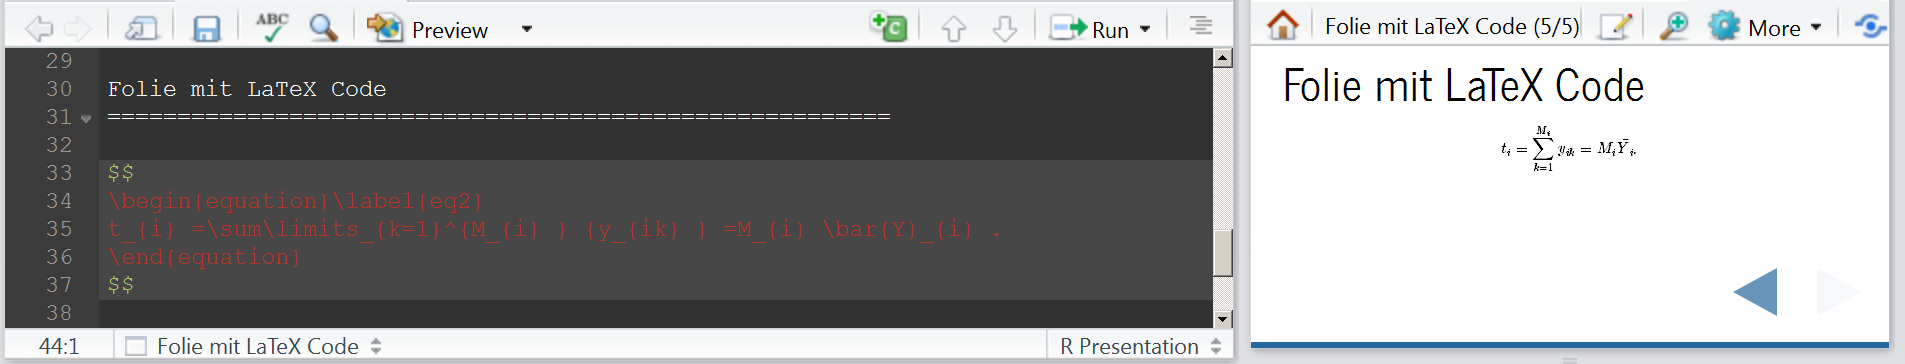
\includegraphics{figure/FolieLatexCode.PNG}
\caption{}
\end{figure}

\subsection{Zwei Spalten}\label{zwei-spalten}

\begin{verbatim}
Folie mit zwei Spalten
====================================
Erste Spalte
***
Zweite Spalte
\end{verbatim}

\subsection{Folienübergänge}\label{folienubergange}

\begin{verbatim}
transition: rotate
\end{verbatim}

\begin{figure}
\centering
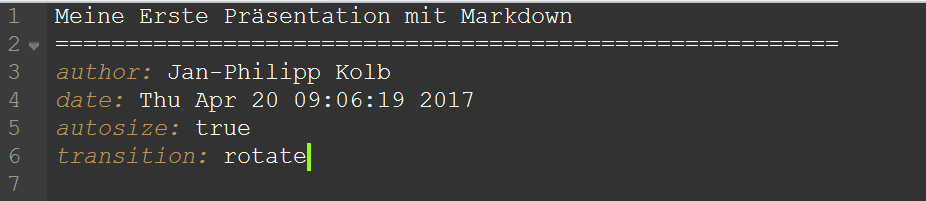
\includegraphics{figure/RpresRotate.PNG}
\caption{}
\end{figure}

\subsection{\texorpdfstring{\href{https://support.rstudio.com/hc/en-us/articles/200714013-Slide-Transitions-and-Navigation}{\textbf{Weitere
mögliche
Folienübergänge}}}{Weitere mögliche Folienübergänge}}\label{weitere-mogliche-folienubergange}

\begin{itemize}
\tightlist
\item
  none
\item
  linear
\item
  rotate
\item
  fade
\item
  zoom
\item
  concave
\end{itemize}

\subsection{Folientypen}\label{folientypen}

\begin{verbatim}
Ein neues Kapitel einfügen
====================================
type: section
\end{verbatim}

\begin{verbatim}
Anderer Folientyp
====================================
type: prompt
\end{verbatim}

\begin{verbatim}
Noch ein anderer Folientyp
====================================
type: alert
\end{verbatim}

\subsection{\texorpdfstring{\href{https://support.rstudio.com/hc/en-us/articles/200532307}{Die
Schriftart
wechseln**}}{Die Schriftart wechseln**}}\label{die-schriftart-wechseln}

\begin{itemize}
\tightlist
\item
  Die
  \href{https://www.w3schools.com/cssref/css_websafe_fonts.asp}{\textbf{CSS
  Schrifttypen}} können verwendet werden
\end{itemize}

\begin{verbatim}
Meine Präsentation
========================================
author: Jan-Philipp Kolb
font-family: 'Impact'
\end{verbatim}

\subsection{Schrifttypen können auch importiert
werden}\label{schrifttypen-konnen-auch-importiert-werden}

\begin{verbatim}
Meine Präsentation
========================================
author: Jan-Philipp Kolb
font-import: http://fonts.googleapis.com/css?family=Risque
font-family: 'Risque'
\end{verbatim}

\begin{figure}
\centering

\includegraphics{figure/SchriftartRisque.PNG}
\caption{}
\end{figure}

\subsection{Kleineren Text}\label{kleineren-text}

Normale Schriftgröße

\begin{verbatim}
<small>This sentence will appear smaller.</small>
\end{verbatim}

\subsection{Die Präsentation
anschauen}\label{die-prasentation-anschauen}

\begin{itemize}
\tightlist
\item
  Das Ergebnis ist hier zu sehen:
\end{itemize}

\url{http://rpubs.com/Japhilko82/FirstRpubs}

\begin{figure}
\centering
\includegraphics{https://support.rstudio.com/hc/en-us/article_attachments/202008388/Screen_Shot_2015-06-04_at_3.51.21_PM.png}
\caption{}
\end{figure}

\section{Eine ioslides Präsentation}\label{eine-ioslides-prasentation}

\subsection{Eine ioslides
Präsentation}\label{eine-ioslides-prasentation-1}

\begin{figure}
\centering

\includegraphics{figure/ioslidespres.PNG}
\caption{}
\end{figure}

\subsection{\texorpdfstring{\href{http://rmarkdown.rstudio.com/ioslides_presentation_format.html}{\textbf{ioslides
- Der Start}}}{ioslides - Der Start}}\label{ioslides---der-start}

\begin{figure}
\centering
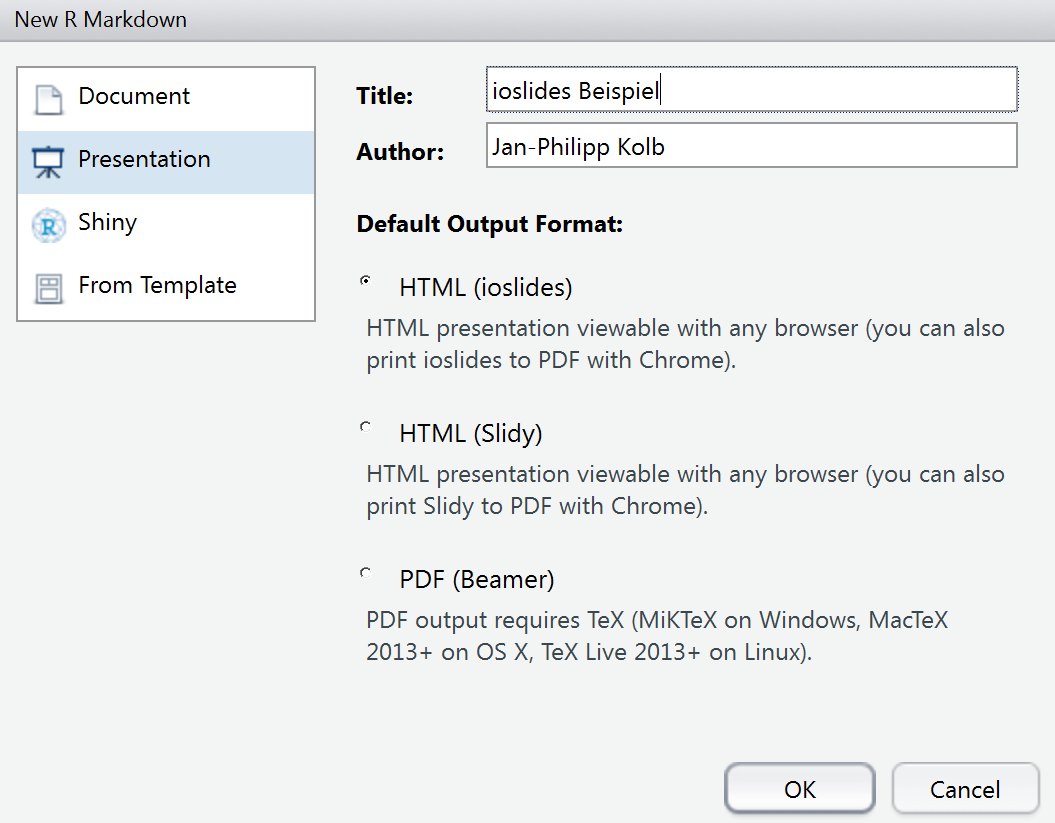
\includegraphics{figure/ioslidesBSP.PNG}
\caption{}
\end{figure}

\subsection{Weitere Dinge tun}\label{weitere-dinge-tun}

\begin{itemize}
\tightlist
\item
  Ein Bild einbinden
\end{itemize}

\begin{verbatim}
![picture of spaghetti](images/spaghetti.jpg)
\end{verbatim}

\subsection{Ein Logo hinzu}\label{ein-logo-hinzu}

\begin{verbatim}
---
title: "ioslides Beispiel"
author: "Jan-Philipp Kolb"
date: "20 April 2017"
output: 
  ioslides_presentation:
    logo: figure/Rlogo.png
---
\end{verbatim}

\begin{figure}
\centering
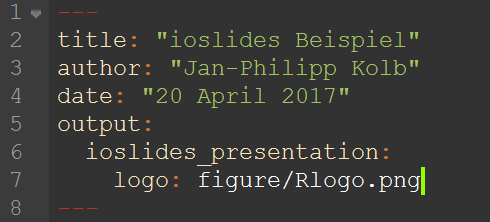
\includegraphics{figure/ioslidesRlogo.PNG}
\caption{}
\end{figure}

\subsection{Tabellen}\label{tabellen}

\begin{itemize}
\tightlist
\item
  Quelle:
  \href{https://www.r-bloggers.com/r-studio-and-presentations-and-git-oh-my/}{\textbf{R
  Studio, and Presentations, and Git! Oh my!}}
\end{itemize}

\begin{Shaded}
\begin{Highlighting}[]
\KeywordTok{library}\NormalTok{(knitr)}
\NormalTok{a <-}\StringTok{ }\KeywordTok{data.frame}\NormalTok{(}\DataTypeTok{a=}\DecValTok{1}\OperatorTok{:}\DecValTok{10}\NormalTok{,}\DataTypeTok{b=}\DecValTok{10}\OperatorTok{:}\DecValTok{1}\NormalTok{)}
\KeywordTok{kable}\NormalTok{(}\KeywordTok{table}\NormalTok{(a))}
\end{Highlighting}
\end{Shaded}

\begin{longtable}[]{@{}rrrrrrrrrr@{}}
\toprule
1 & 2 & 3 & 4 & 5 & 6 & 7 & 8 & 9 & 10\tabularnewline
\midrule
\endhead
0 & 0 & 0 & 0 & 0 & 0 & 0 & 0 & 0 & 1\tabularnewline
0 & 0 & 0 & 0 & 0 & 0 & 0 & 0 & 1 & 0\tabularnewline
0 & 0 & 0 & 0 & 0 & 0 & 0 & 1 & 0 & 0\tabularnewline
0 & 0 & 0 & 0 & 0 & 0 & 1 & 0 & 0 & 0\tabularnewline
0 & 0 & 0 & 0 & 0 & 1 & 0 & 0 & 0 & 0\tabularnewline
0 & 0 & 0 & 0 & 1 & 0 & 0 & 0 & 0 & 0\tabularnewline
0 & 0 & 0 & 1 & 0 & 0 & 0 & 0 & 0 & 0\tabularnewline
0 & 0 & 1 & 0 & 0 & 0 & 0 & 0 & 0 & 0\tabularnewline
0 & 1 & 0 & 0 & 0 & 0 & 0 & 0 & 0 & 0\tabularnewline
1 & 0 & 0 & 0 & 0 & 0 & 0 & 0 & 0 & 0\tabularnewline
\bottomrule
\end{longtable}

\subsection{\texorpdfstring{\texttt{knitr}
Engines}{knitr Engines}}\label{knitr-engines}

\begin{itemize}
\item
  \href{http://rmarkdown.rstudio.com/authoring_knitr_engines.html}{\textbf{knitr
  Language Engines}}
\item
  \href{http://slidify.org/}{\textbf{slidify}}
\end{itemize}

\section{Eine slidy Präsentation}\label{eine-slidy-prasentation}

\subsection{slidy Präsentationen}\label{slidy-prasentationen}

\begin{figure}
\centering

\includegraphics{figure/sluidypresentations.PNG}
\caption{}
\end{figure}

\subsection{\texorpdfstring{{[}**Was sind Cascading Style Files
(\href{https://de.wikipedia.org/wiki/Cascading_Style_Sheets}{CSS**})}{{[}**Was sind Cascading Style Files (CSS**)}}\label{was-sind-cascading-style-files-css}

\begin{figure}
\centering
\includegraphics{https://upload.wikimedia.org/wikipedia/commons/8/83/CSS-Logo.png}
\caption{}
\end{figure}

\begin{itemize}
\tightlist
\item
  Stylesheet-Sprache für elektronische Dokumente
\item
  eine der Kernsprachen des World Wide Webs.
\item
  CSS wurde entworfen, um Darstellungsvorgaben weitgehend von den
  Inhalten zu trennen
\end{itemize}

\subsubsection{CSS und R}\label{css-und-r}

\begin{itemize}
\tightlist
\item
  \href{http://rmarkdown.rstudio.com/html_document_format.html\#custom_css}{\textbf{Custom
  CSS}}
\item
  \href{https://github.com/AllThingsSmitty/css-protips\#use-a-css-reset}{\textbf{CSS
  pro tipps}}
\end{itemize}

\subsection{Beispiel CSS}\label{beispiel-css}

\begin{figure}
\centering
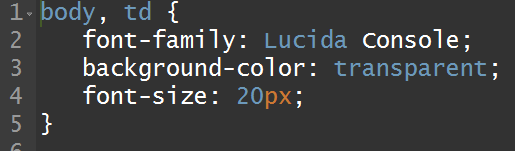
\includegraphics{figure/cssRstudio.PNG}
\caption{}
\end{figure}

\subsection{Das CSS ändern}\label{das-css-andern}

Um den Präsentationstyp zu ändern kann man das CSS verändern

\begin{itemize}
\item
  \href{https://de.wikipedia.org/wiki/Cascading_Style_Sheets}{\textbf{Cascading
  Style Sheets}} (CSS)
\item
  Bspw. lässt sich die
  \href{http://tomheller.de/html-farben.html}{\textbf{Farbe (HTML)}}
  ändern.
\item
  \href{https://www.mediaevent.de/css/font-family.html}{\textbf{Man kann
  eine andere Schriftart wählen}}
\item
  \href{https://wiki.selfhtml.org/wiki/CSS/Eigenschaften/Schriftformatierung}{\textbf{Es
  gibt zahlreiche Möglichkeiten der Schriftformatierung}}
\item
  Daneben gibt es viele weitere Dinge,
  \href{https://www.w3.org/TR/WCAG20-TECHS/C22.html}{\textbf{die sich
  mit dem CSS steuern lassen}}
\end{itemize}

\section{HTML Dokumente}\label{html-dokumente}

\subsection{Ein HTML Dokument
erzeugen}\label{ein-html-dokument-erzeugen}

\begin{figure}
\centering
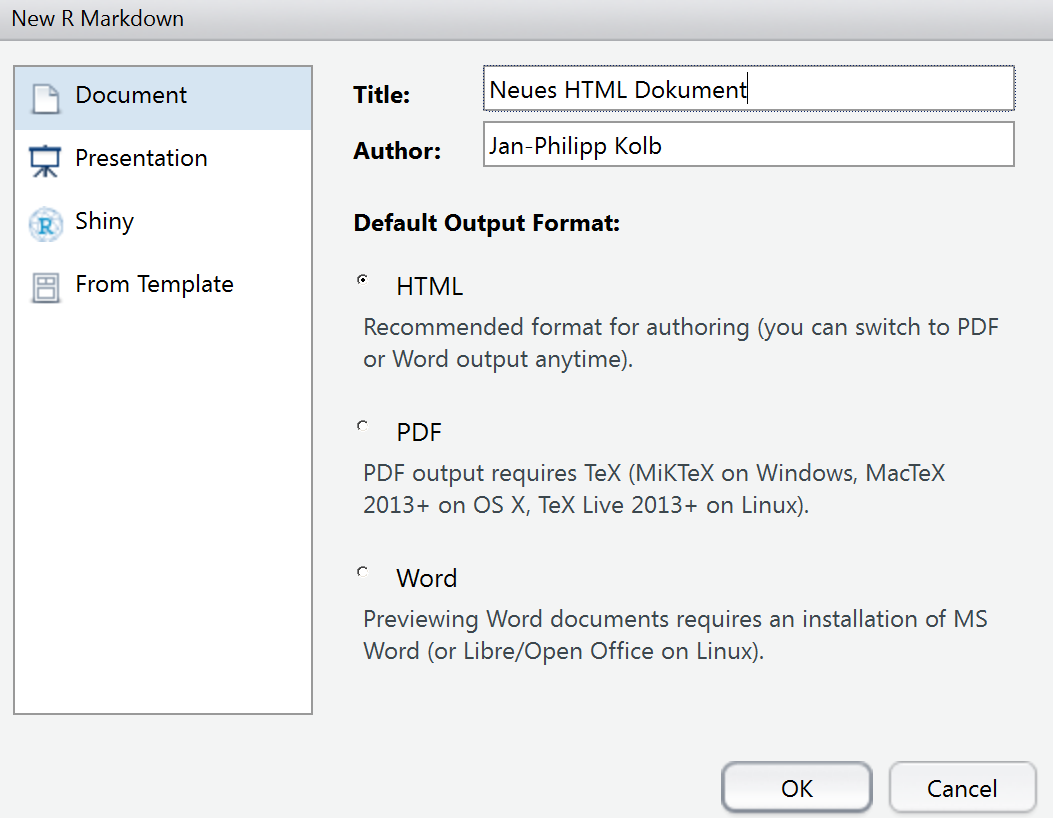
\includegraphics{figure/NewHTML.PNG}
\caption{}
\end{figure}

\subsection{Ein Template verwenden}\label{ein-template-verwenden}

\begin{figure}
\centering
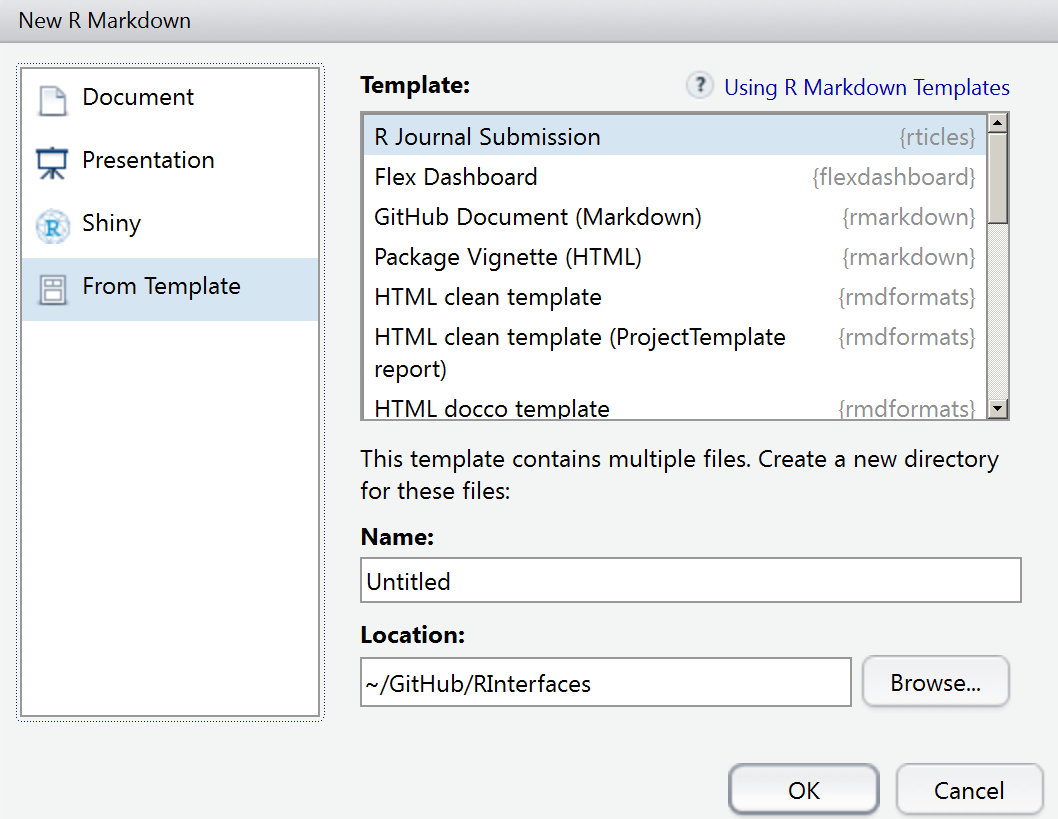
\includegraphics{figure/UsingTemplate.PNG}
\caption{}
\end{figure}

\subsection{\texorpdfstring{\href{http://rmarkdown.rstudio.com/developer_document_templates.html}{\textbf{Weitere
Vorlagen
nutzen}}}{Weitere Vorlagen nutzen}}\label{weitere-vorlagen-nutzen}

\begin{itemize}
\tightlist
\item
  Es gibt viele Formate -
  \href{https://blog.rstudio.org/2016/03/21/r-markdown-custom-formats/}{\textbf{manche
  müssen erst aktiviert werden}}:
\end{itemize}

\begin{Shaded}
\begin{Highlighting}[]
\KeywordTok{install.packages}\NormalTok{(}\StringTok{"rticles"}\NormalTok{)}
\end{Highlighting}
\end{Shaded}

\begin{figure}
\centering

\includegraphics{figure/ShortPaper.PNG}
\caption{}
\end{figure}

\subsection{Vorlagen für Markdown}\label{vorlagen-fur-markdown}

Das Paket \texttt{rmdformats} - HTML Output Formats and Templates for
`rmarkdown'

\begin{Shaded}
\begin{Highlighting}[]
\KeywordTok{install.packages}\NormalTok{(}\StringTok{"rmdformats"}\NormalTok{)}
\end{Highlighting}
\end{Shaded}

\begin{itemize}
\tightlist
\item
  \texttt{ProjectTemplate} - Automates the Creation of New Statistical
  Analysis
\end{itemize}

\begin{Shaded}
\begin{Highlighting}[]
\KeywordTok{install.packages}\NormalTok{(}\StringTok{"ProjectTemplate"}\NormalTok{)}
\end{Highlighting}
\end{Shaded}

\begin{itemize}
\tightlist
\item
  \texttt{tufte} - Tufte's Styles for R Markdown Documents
\end{itemize}

\begin{Shaded}
\begin{Highlighting}[]
\KeywordTok{install.packages}\NormalTok{(}\StringTok{"tufte"}\NormalTok{)}
\end{Highlighting}
\end{Shaded}

\subsection{\texorpdfstring{\href{https://github.com/juba/rmdformats}{\textbf{Beispiele
für
Templates}}}{Beispiele für Templates}}\label{beispiele-fur-templates}

\begin{figure}
\centering
\includegraphics{https://rstudioblog.files.wordpress.com/2016/03/readthedown.png}
\caption{}
\end{figure}

\section{Dashboards}\label{dashboards}

\subsection{\texorpdfstring{\href{https://gallery.shinyapps.io/cran-gauge/}{\textbf{Beispiel
R-Pakete}}}{Beispiel R-Pakete}}\label{beispiel-r-pakete}

\begin{figure}
\centering
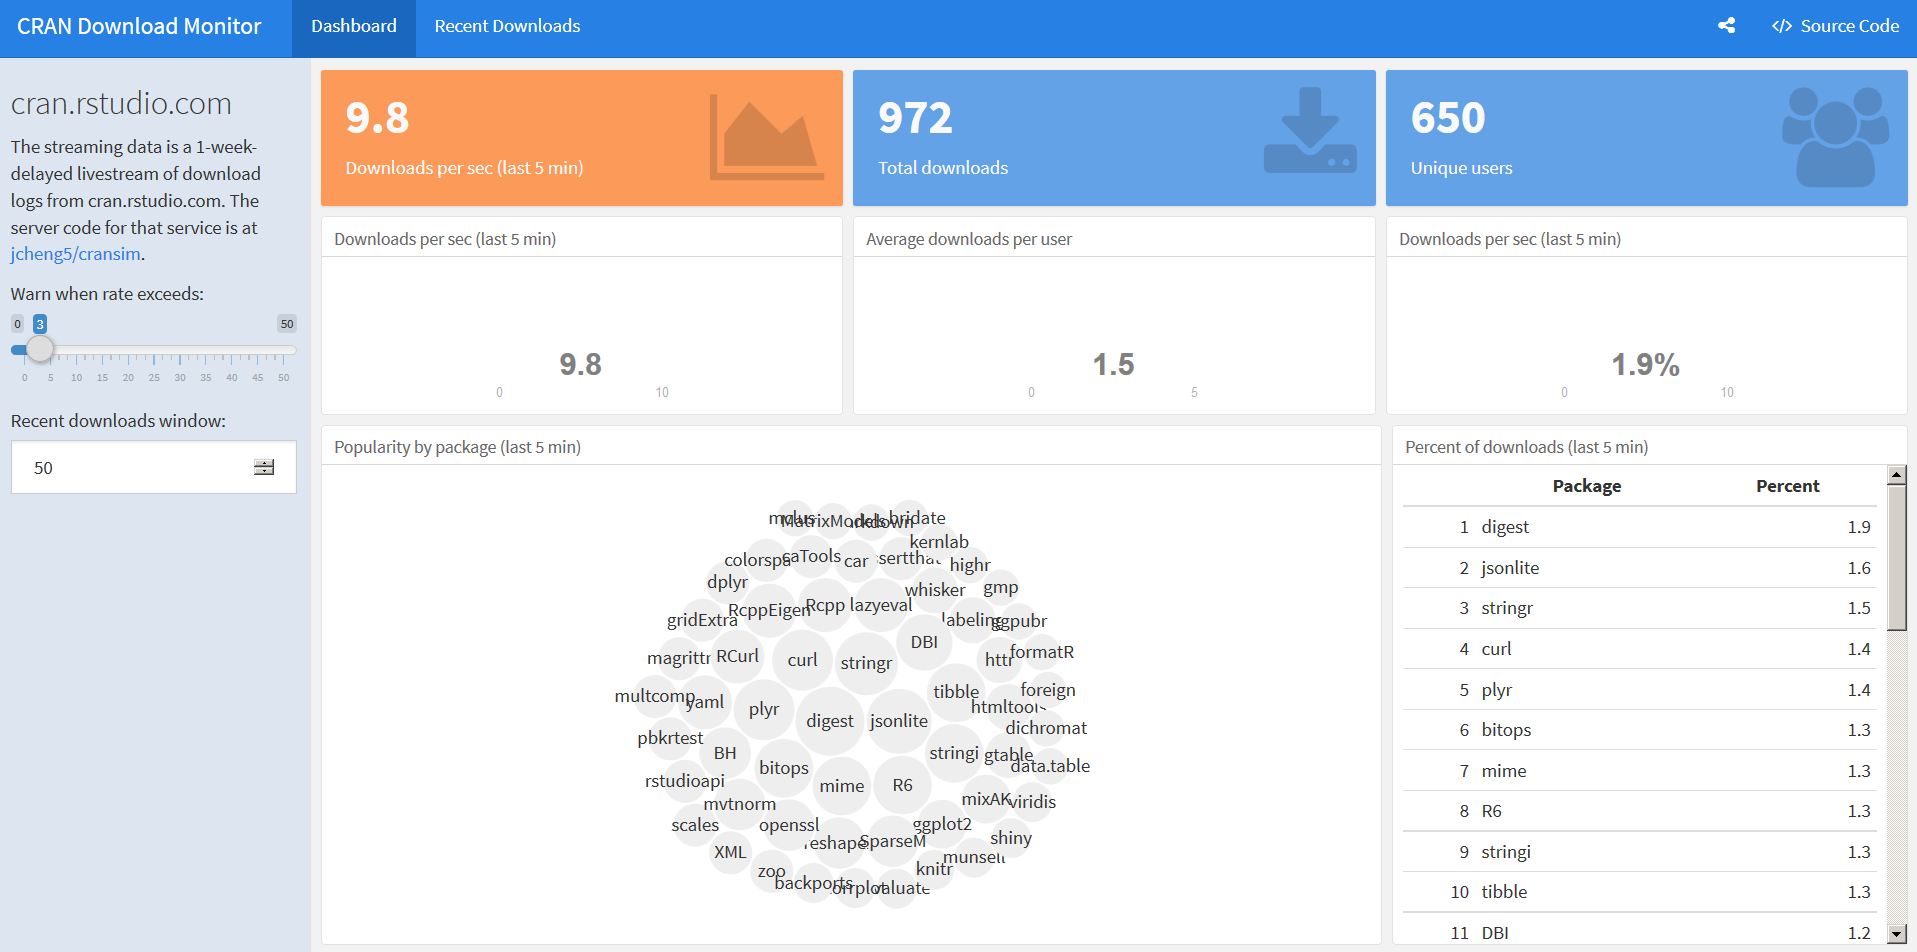
\includegraphics{figure/CRANdownloads.PNG}
\caption{}
\end{figure}

\subsection{\texorpdfstring{\href{https://blog.rstudio.org/2016/05/17/flexdashboard-easy-interactive-dashboards-for-r/}{\textbf{Paket
installieren}}}{Paket installieren}}\label{paket-installieren}

\begin{Shaded}
\begin{Highlighting}[]
\KeywordTok{install.packages}\NormalTok{(}\StringTok{"flexdashboard"}\NormalTok{, }\DataTypeTok{type =} \StringTok{"source"}\NormalTok{)}
\end{Highlighting}
\end{Shaded}

\begin{figure}
\centering
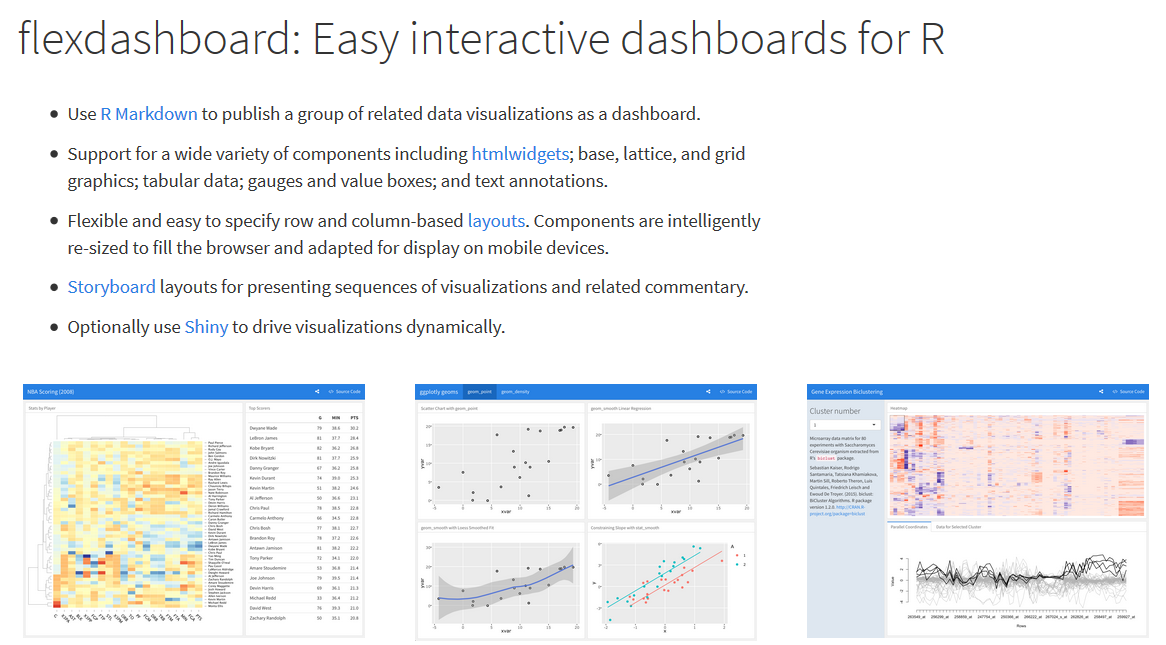
\includegraphics{figure/flexdashboards.PNG}
\caption{}
\end{figure}

\subsection{Ein Dashboard erstellen mit
Rstudio}\label{ein-dashboard-erstellen-mit-rstudio}

\begin{figure}
\centering
\includegraphics{https://i2.wp.com/rmarkdown.rstudio.com/flexdashboard/images/NewRMarkdown.png?zoom=2}
\caption{}
\end{figure}

\subsection{\texorpdfstring{\href{http://rpubs.com/Japhilko82/whcsites}{\textbf{Mein
erstes Dashboard}}}{Mein erstes Dashboard}}\label{mein-erstes-dashboard}

\begin{figure}
\centering
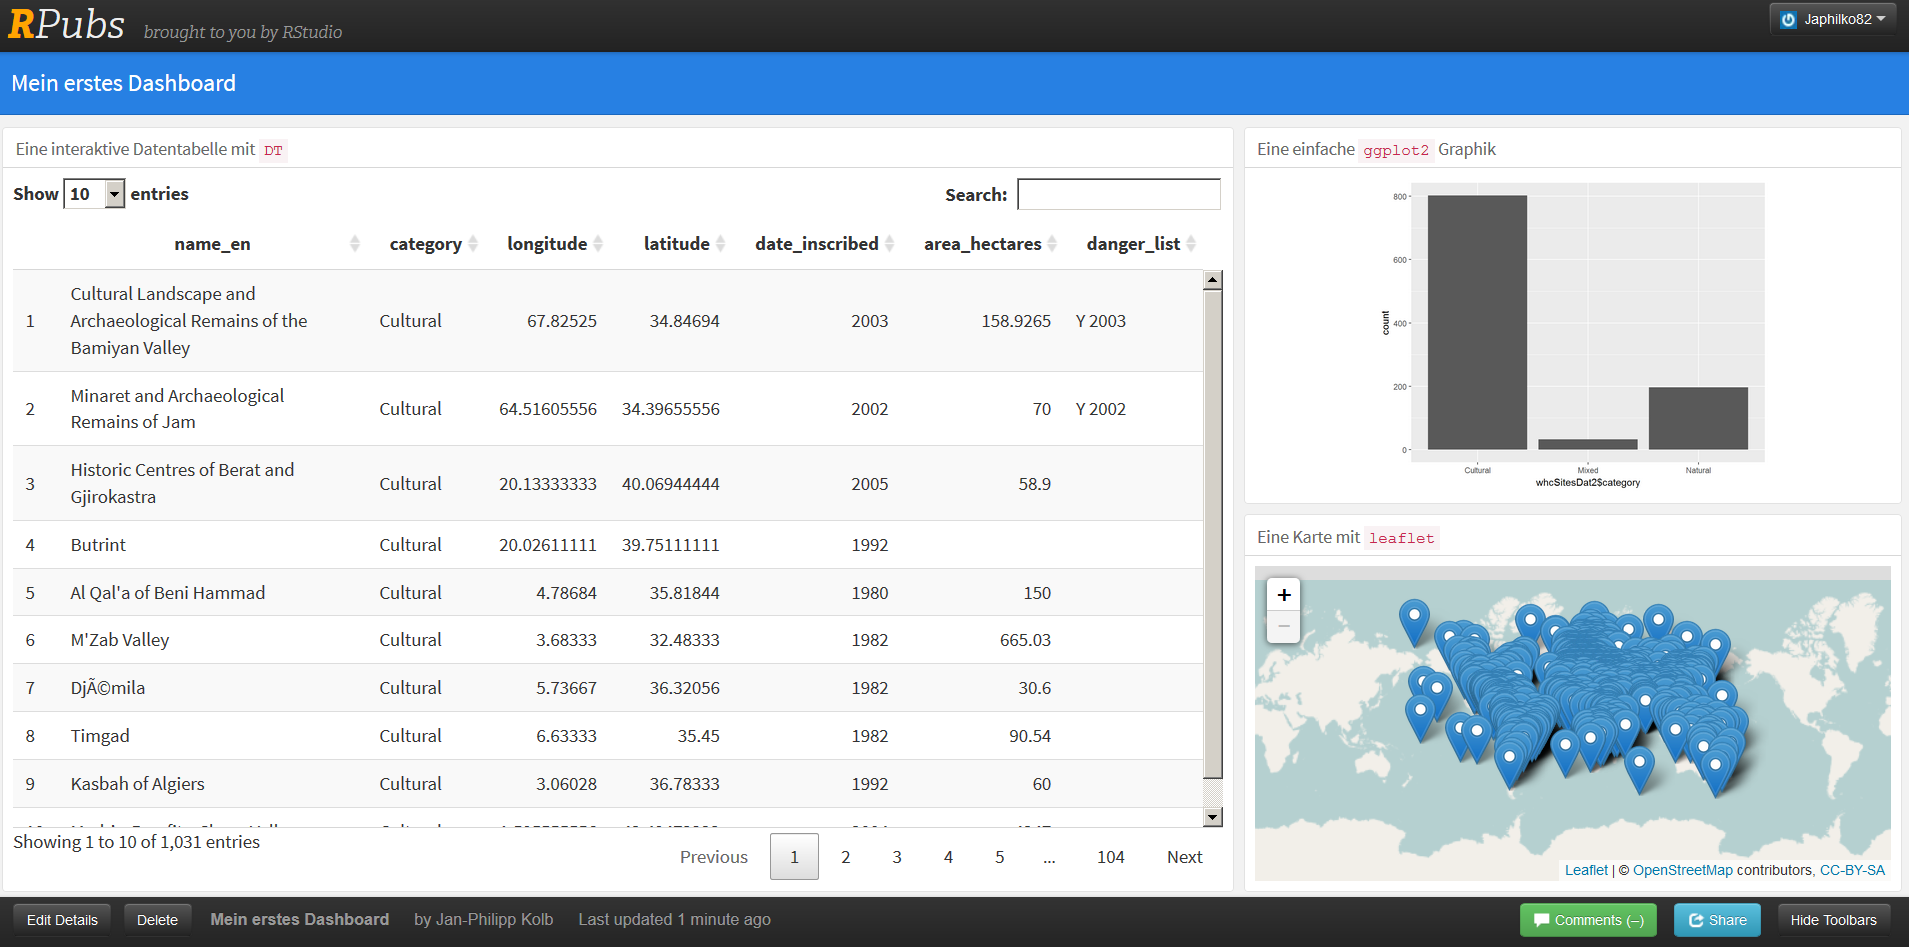
\includegraphics{figure/MeinErstesDashboard.PNG}
\caption{}
\end{figure}

\subsection{\texorpdfstring{\href{http://rmarkdown.rstudio.com/gallery.html}{\textbf{Gallerie}}}{Gallerie}}\label{gallerie}

\begin{figure}
\centering
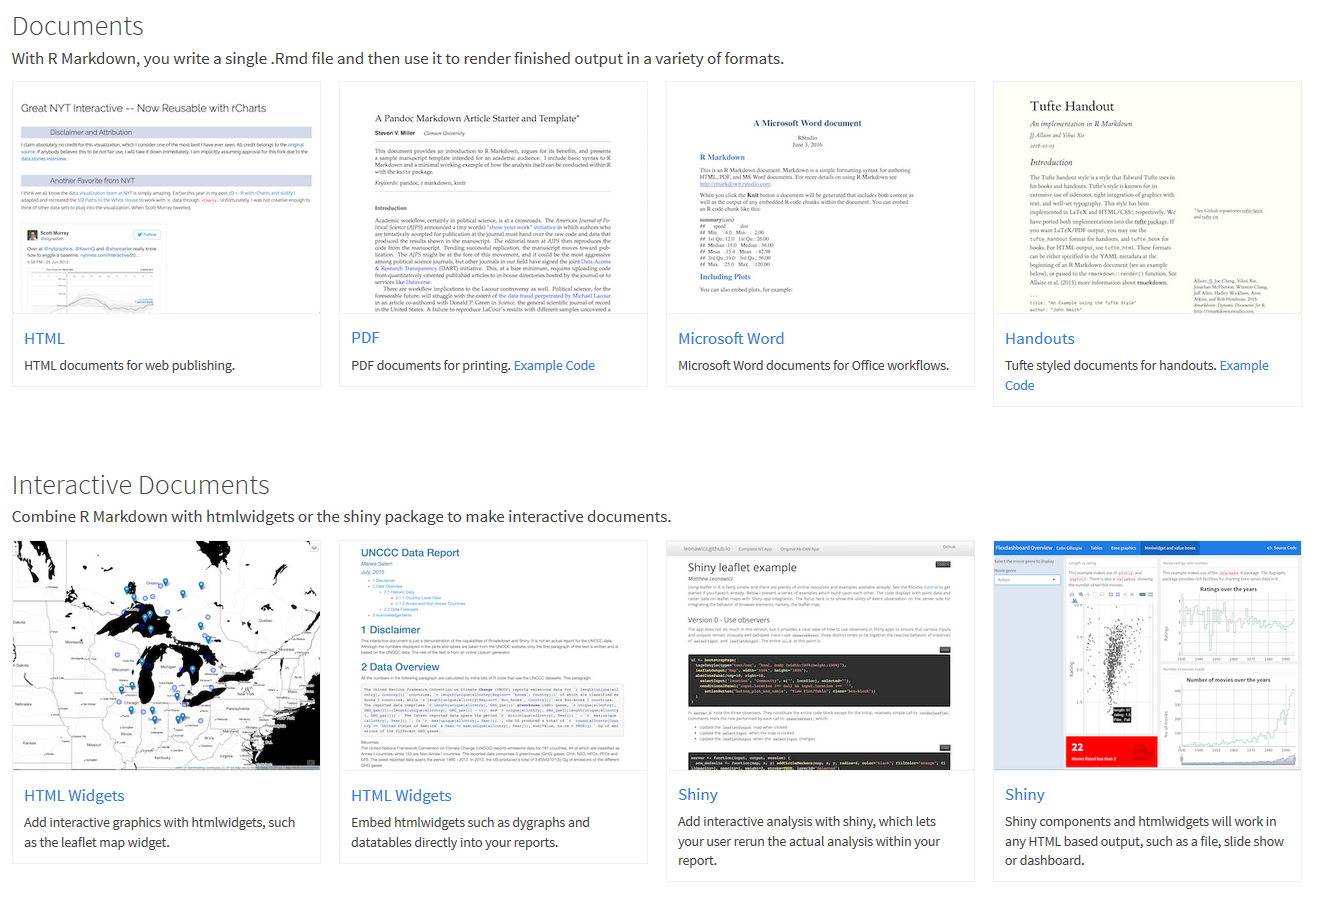
\includegraphics{figure/RmarkdownGallery.PNG}
\caption{}
\end{figure}

\subsection{Links}\label{links}

\begin{itemize}
\tightlist
\item
  \href{http://rmarkdown.rstudio.com/formats.html}{\textbf{Formate}}
\item
  \href{http://stackoverflow.com/questions/25824795/how-to-combine-two-rmarkdown-rmd-files-into-a-single-output}{\textbf{Verschiedene
  Markdown Dokumente zusammen fügen}}
\end{itemize}

\begin{figure}
\centering
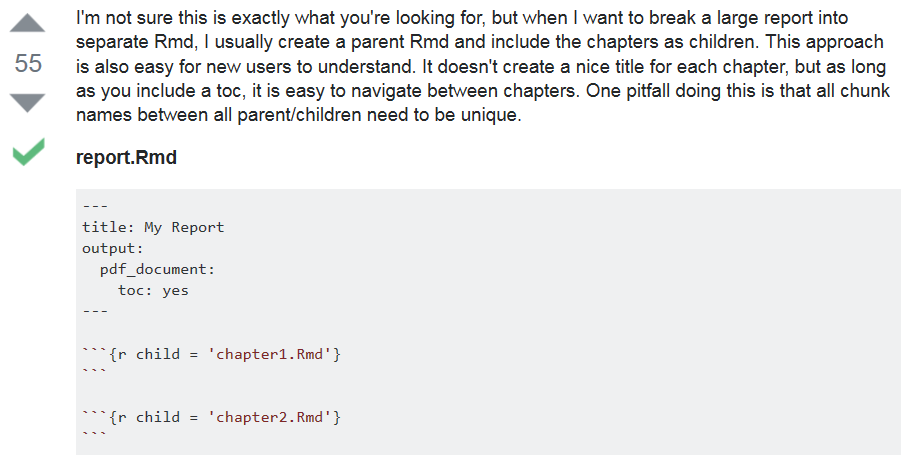
\includegraphics{figure/stackoverflowCombine.PNG}
\caption{}
\end{figure}

\begin{itemize}
\item
  \href{http://www.cssfontstack.com/}{\textbf{Verschiedene CSS Fonts}}
\item
  {[}Überblick über die verschiedenen Rmarkdown
\end{itemize}


\end{document}
